\chapter{Introduction}
	%  - Introduction 
			%- 	CMB 
			%- 	Cosmological Parameters
\section{The Cosmic Microwave Background}
The basis for modern cosmology relies on several fundamental assumptions stemming from observation, the chief of which is the Big Bang Model. Following Hubble's discovery of a relation between distances to galaxies and their recessional velocities, the \emph{Copernican Principle} leads to the conclusion that in the past, objects in the universe were much closer together. His observations gave rise to the Lemaitre's Hubble Law,
\begin{equation}
	v  \varpropto d
	\label{eq:HubbleLaw}
\end{equation}
This suggests that at some point in the past, the universe was much smaller than it is at present, the conservation of energy then implies that at some point in the past, the universe must have been an incredibly hot, dense environment. Using general relativity, the extrapolation backwards in time yields a singularity of infinite density and temperature, which is commonly called the \emph{Big Bang}
\par Another assumption stemming from observation is that of isotropy. Based on observation, there appears to be no favoured direction in the universe, since distributions of distant galaxies and other extragalactic sources seem to be evenly distributed across the sky. Perhaps the most spectacular example of this isotropy is the presence of the \emph{Cosmic Microwave Background}.
\par Discovered in 1964 \citep{Penzias:65}, it was noticed that there was isotropic black-body radiation at $T \approx \SI{2.7}{\kelvin}$. Since the peak of this radiation is in the microwave section of the electromagnetic spectrum, it was termed the \emph{Cosmic Microwave Background}.
\begin{figure}[ht]
	\centering
	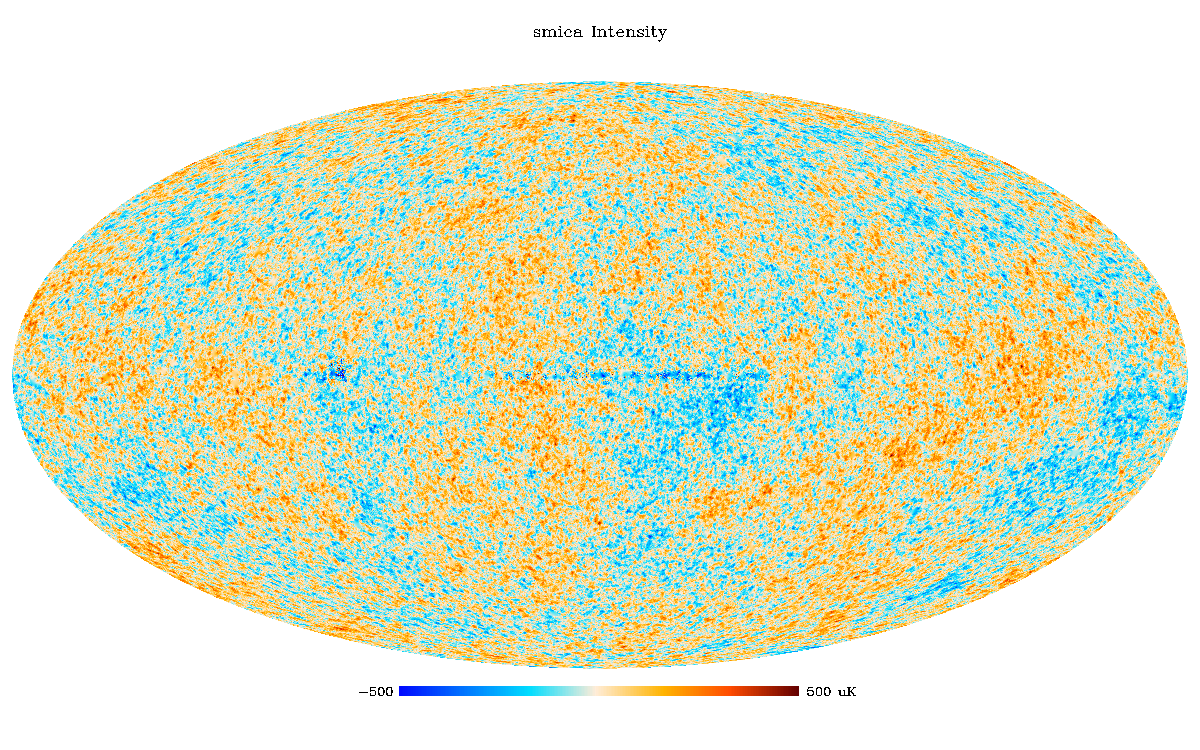
\includegraphics[scale=0.25]{/home/mitchell/Documents/masters/masters/thesis/Images/CMB_smica_tsig.png}
	\label{CMB Map}
	\caption{\emph{Planck} Satellite Full Sky CMB Map}
\end{figure}

The Cosmic Microwave Background (CMB) provides the most accurate and detailed measures of the primary cosmological parameters to date. 

\section{Cosmological Parameters}
For a $\Lambda$ CDM universe, there are six independant paramters which descirbe the evolution and behaviour of the universe, the physical baryon density $\Omega_b h^2$, the physical dark matter density $\Omega_c h^2$, the age of the universe $t_0$ (or its reciprocal, the Hubble constant $H_0$), the scalar spectral index $n_s$, the curvature fluctuation amplitude $\Delta_R^2$, and the reionisation optical depth $\tau$. 

Currently, the highest precision measures of these features from the CMB come from \cite{2018arXiv180706209P}, which details that baryonic matter only comprises $\approx 5 \% $ of the universe's energy density. In principle, this component of the universe should be directly measurable. At just three minutes after the Big Bang, deuterium can be used as a tracer for this abundance \citep{2007ARNPS..57..463S}, and at redshift $z \geqslant 2$, the baryon fraction can be found in the absorption lines of quasars passing through the diffuse, photo-ionised intergalactic medium, known as the Lyman-$\alpha$ forest \citep{1997ApJ...490..564W}. However as the universe evolved, this gas became sparser as it became more ionised. This makes searching for the entirety of the baryon fraction at low redshift difficult. When this fraction is calculated directly from observations, it shows only one tenth of the baryonic content shown in high redshift measurements is contained in galactic structures \citep{1992MNRAS.258P..14P}. Some revised estimates considered that the limitations of observations were primarily to blame for this discrepency, and not inherent new physics \citep{1994MNRAS.267...13B, 1998ApJ...503..518F}

The baryon content has been confirmed to a very high accuracy with recent CMB experiments, first with the \textit{Wilkinson Microwave Anisotropy Probe} (WMAP) \citep{2007ApJS..170..377S}, and then with the \textit{Planck} Satellite \citep{2018arXiv180706209P}. When we quote quantities, we take values from the latest \textit{Planck} paper


\begin{center}\label{table:params}
 \begin{tabular}{||c c c||} 
 \hline
 Parameter & Value & Error \\
 \hline\hline
 $\Omega_c h^2$ & $0.120$ & $\pm 0.001$ \\
 \hline
 $\Omega_b h^2$ & $0.0224$ & $\pm 0.0001$ \\
 \hline
  $n_s$ & $0.965$ & $\pm 0.004$ \\
 \hline
  $\tau$  & $0.054$ & $\pm 0.007$ \\
 \hline
  $100 \Theta_\star$ & $1.0411$ & $\pm 0.0003$ \\
 \hline
 $H_0$ (km s$^{-1}$ Mpc$^{-1}$) & $67.4$ & $\pm 0.5$ \\
 \hline
\end{tabular}
\end{center}



